\documentclass[11pt,a4paper]{article}

\usepackage[a4paper,margin=0.75in,top=1.05in,bottom=0.78in,headheight=39pt,headsep=14pt,footskip=25pt]{geometry}
\usepackage[utf8]{inputenc}
\usepackage[T1]{fontenc}
\usepackage{lmodern}
\usepackage{amsmath,amssymb,mathtools}
\usepackage{booktabs,array,longtable,tabularx}
\usepackage{fancyhdr}
\usepackage{xcolor}
\usepackage{enumitem}
\usepackage{graphicx}
\usepackage{tikz}
\usepackage{pgfplots}
\usepackage{float}
\usepackage[font=small,labelfont=bf]{caption}
\usepackage[hidelinks]{hyperref}
\usetikzlibrary{arrows.meta,positioning,calc,trees}
\pgfplotsset{compat=1.18}

\newcommand{\StudentName}{Shourya Veer Singh}
\newcommand{\RegistrationNumber}{24118105}
\newcommand{\supp}{\operatorname{supp}}
\newcommand{\conf}{\operatorname{conf}}
\newcommand{\Lift}{\operatorname{Lift}}

\setlength{\parindent}{0pt}
\setlength{\parskip}{3pt}
\setlength{\tabcolsep}{5pt}
\renewcommand{\arraystretch}{1.12}
\setlist[enumerate]{leftmargin=1.7em,itemsep=1pt,topsep=2pt}
\setlist[itemize]{leftmargin=1.5em,itemsep=1pt,topsep=2pt}
\setcounter{secnumdepth}{0}

\pagestyle{fancy}
\fancyhf{}
\fancyhead[R]{%
  \begin{tabular}{@{}r@{}}
    \small\textbf{Name: \StudentName}\\[-1pt]
    \small Registration No.: \RegistrationNumber\\[-1pt]
    \small Signature: \rule{2.1cm}{0.4pt}
  \end{tabular}}
\fancyfoot[C]{\small Data Mining -- Assignment-II}
\fancyfoot[R]{\small\thepage}
\renewcommand{\headrulewidth}{0.4pt}
\renewcommand{\footrulewidth}{0pt}
\fancypagestyle{plain}{%
  \fancyhf{}
  \fancyhead[R]{%
    \begin{tabular}{@{}r@{}}
      \small\textbf{Name: \StudentName}\\[-1pt]
      \small Registration No.: \RegistrationNumber\\[-1pt]
      \small Signature: \rule{2.1cm}{0.4pt}
    \end{tabular}}
  \fancyfoot[C]{\small Data Mining -- Assignment-II}
  \fancyfoot[R]{\small\thepage}
  \renewcommand{\headrulewidth}{0.4pt}
}
\fancypagestyle{cover}{%
  \fancyhf{}
  \fancyhead[R]{%
    \begin{tabular}{@{}r@{}}
      \small\textbf{Name: \StudentName}\\[-1pt]
      \small Registration No.: \RegistrationNumber\\[-1pt]
      \small Signature: \rule{2.1cm}{0.4pt}
    \end{tabular}}
  \fancyfoot[C]{\small Data Mining -- Assignment-II}
  \renewcommand{\headrulewidth}{0.4pt}
  \renewcommand{\footrulewidth}{0pt}
}

\begin{document}

\begin{titlepage}
\thispagestyle{cover}
\vspace*{1.2cm}
\begin{center}
{\Large\bfseries NATIONAL INSTITUTE OF TECHNOLOGY RAIPUR\par}
\vspace{0.3cm}
{\large Department of Information Technology\par}
\vspace{0.2cm}
{\large B.Tech. -- Fifth Semester\par}
\vspace{0.8cm}
{\large Course: Data Mining\par}
\vspace{0.4cm}
{\LARGE\bfseries ASSIGNMENT-II\par}
\end{center}
\vfill
\begin{center}
\renewcommand{\arraystretch}{1.5}
\begin{tabular}{|>{\bfseries}p{4.2cm}|p{8.0cm}|}
\hline
Student Name & \StudentName\\ \hline
Registration Number & \RegistrationNumber\\ \hline
Signature & \rule{5.5cm}{0.4pt}\\ \hline
\end{tabular}
\end{center}
\vfill
\end{titlepage}
\setcounter{page}{1}

\section*{Question 1. K-Means and Agglomerative Clustering}

\subsection*{(a) K-means with \(k=2\)}
Because initial centroids are not specified, use the deterministic data-point initialization
\(\mu_1^{(0)}=a=(2,0)\) and \(\mu_2^{(0)}=j=(3,5)\).
Distances below are squared Euclidean distances; each point is assigned to the nearer centroid.

\begin{center}
\small
\begin{tabular}{c|r r|c}
\toprule
Point & \(d^2(\mu_1^{(0)})\) & \(d^2(\mu_2^{(0)})\) & Iteration 1\\
\midrule
a & 0 & 26 & \(C_1\)\\
b & 5 & 13 & \(C_1\)\\
c & 4 & 10 & \(C_1\)\\
d & 5 & 9 & \(C_1\)\\
e & 9 & 5 & \(C_2\)\\
f & 10 & 4 & \(C_2\)\\
g & 16 & 2 & \(C_2\)\\
h & 17 & 1 & \(C_2\)\\
i & 20 & 2 & \(C_2\)\\
j & 26 & 0 & \(C_2\)\\
\bottomrule
\end{tabular}
\end{center}

After iteration 1,
\[
C_1^{(1)}=\{a,b,c,d\},\qquad C_2^{(1)}=\{e,f,g,h,i,j\}.
\]
The updated centroids are
\[
\mu_1^{(1)}=\left(\frac{2+1+2+3}{4},\frac{0+2+2+2}{4}\right)
=(2,1.5),
\]
\[
\mu_2^{(1)}=\left(\frac{17}{6},\frac{23}{6}\right)
\approx(2.8333,3.8333).
\]
Reassignment using these updated centroids gives the same clusters:

\begin{center}
\small
\begin{tabular}{c|r r|c}
\toprule
Point & \(d^2(\mu_1^{(1)})\) & \(d^2(\mu_2^{(1)})\) & Iteration 2\\
\midrule
a & 2.250 & 15.389 & \(C_1\)\\
b & 1.250 & 6.722 & \(C_1\)\\
c & 0.250 & 4.056 & \(C_1\)\\
d & 1.250 & 3.389 & \(C_1\)\\
e & 2.250 & 1.389 & \(C_2\)\\
f & 3.250 & 0.722 & \(C_2\)\\
g & 6.250 & 0.722 & \(C_2\)\\
h & 7.250 & 0.056 & \(C_2\)\\
i & 10.250 & 1.389 & \(C_2\)\\
j & 13.250 & 1.389 & \(C_2\)\\
\bottomrule
\end{tabular}
\end{center}
There is no reassignment, so the algorithm has converged. The final clusters and centroids are
\[
C_1=\{a,b,c,d\},\quad \mu_1=(2,1.5);
\qquad
C_2=\{e,f,g,h,i,j\},\quad \mu_2=\left(\frac{17}{6},\frac{23}{6}\right).
\]
The within-cluster sum of squared errors is
\[
\begin{aligned}
\operatorname{SSE}(C_1)
&=2.25+1.25+0.25+1.25=5,\\
\operatorname{SSE}(C_2)
&=\frac{25+13+13+1+25+25}{18}
=\frac{17}{3}\approx5.6667,\\
\operatorname{SSE}_{\mathrm{total}}
&=5+\frac{17}{3}=\boxed{\frac{32}{3}\approx10.6667}.
\end{aligned}
\]

\begin{figure}[H]
\centering
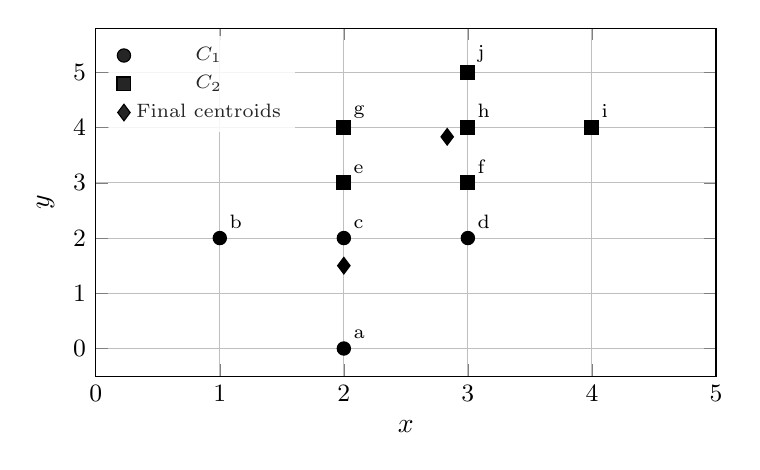
\begin{tikzpicture}
\begin{axis}[
  width=0.78\linewidth,height=6.0cm,
  xmin=0,xmax=5,ymin=-0.5,ymax=5.8,
  xtick={0,1,2,3,4,5},ytick={0,1,2,3,4,5},
  xlabel=\(x\),ylabel=\(y\),grid=major,
  legend style={at={(0.02,0.98)},anchor=north west,font=\scriptsize,
    draw=none,fill=white,fill opacity=0.85},
  tick label style={font=\small}
]
\addplot[only marks,mark=*,mark size=2.4pt] coordinates
  {(2,0)(1,2)(2,2)(3,2)};
\addlegendentry{\(C_1\)}
\addplot[only marks,mark=square*,mark size=2.5pt] coordinates
  {(2,3)(3,3)(2,4)(3,4)(4,4)(3,5)};
\addlegendentry{\(C_2\)}
\addplot[only marks,mark=diamond*,mark size=3pt] coordinates
  {(2,1.5)(2.8333,3.8333)};
\addlegendentry{Final centroids}
\node[font=\scriptsize,anchor=south west] at (axis cs:2,0) {a};
\node[font=\scriptsize,anchor=south west] at (axis cs:1,2) {b};
\node[font=\scriptsize,anchor=south west] at (axis cs:2,2) {c};
\node[font=\scriptsize,anchor=south west] at (axis cs:3,2) {d};
\node[font=\scriptsize,anchor=south west] at (axis cs:2,3) {e};
\node[font=\scriptsize,anchor=south west] at (axis cs:3,3) {f};
\node[font=\scriptsize,anchor=south west] at (axis cs:2,4) {g};
\node[font=\scriptsize,anchor=south west] at (axis cs:3,4) {h};
\node[font=\scriptsize,anchor=south west] at (axis cs:4,4) {i};
\node[font=\scriptsize,anchor=south west] at (axis cs:3,5) {j};
\end{axis}
\end{tikzpicture}
\caption{Final K-means clusters and centroids using the stated initialization.}
\label{fig:kmeans}
\end{figure}

\subsection*{(b) Agglomerative clustering on \(a,b,c,d,e,f\)}
Use Euclidean distance with \textbf{single linkage}: the distance between two clusters is the minimum pairwise distance between their points. The initial proximity matrix is
\[
\begin{array}{c|rrrrrr}
 & a&b&c&d&e&f\\ \hline
a&0&\sqrt5&2&\sqrt5&3&\sqrt{10}\\
b&\sqrt5&0&1&2&\sqrt2&\sqrt5\\
c&2&1&0&1&1&\sqrt2\\
d&\sqrt5&2&1&0&\sqrt2&1\\
e&3&\sqrt2&1&\sqrt2&0&1\\
f&\sqrt{10}&\sqrt5&\sqrt2&1&1&0
\end{array}
\]
The minimum distance is \(1\), with several ties. Resolve ties deterministically by first choosing the lexicographically earliest point/cluster pair. The successive merges are:
\[
\{b\},\{c\}\xrightarrow{1}\{b,c\},\quad
\{b,c\},\{d\}\xrightarrow{1}\{b,c,d\},\quad
\{b,c,d\},\{e\}\xrightarrow{1}\{b,c,d,e\},
\]
\[
\{b,c,d,e\},\{f\}\xrightarrow{1}\{b,c,d,e,f\},\quad
\{a\},\{b,c,d,e,f\}\xrightarrow{2}\{a,b,c,d,e,f\}.
\]
Thus the tied single-link merges from \(b\) through \(f\) occur at height 1; \(a\) joins at height 2.

\begin{figure}[H]
\centering
\begin{tikzpicture}[x=1.1cm,y=1.25cm]
\draw[->] (-0.5,0)--(-0.5,2.7) node[above] {Distance};
\draw (0,0) node[below=2pt] {a} -- (0,2);
\foreach \x/\lab in {1/b,2/c,3/d,4/e,5/f}
  {\draw (\x,0) node[below=2pt] {\lab} -- (\x,1);}
\draw (1,1)--(5,1);
\draw (3,1)--(3,2);
\draw (0,2)--(3,2);
\draw[dashed] (-0.5,1)--(5.5,1) node[right] {\scriptsize merge height 1};
\draw[dashed] (-0.5,2)--(5.5,2) node[right] {\scriptsize final merge height 2};
\end{tikzpicture}
\caption{Single-link dendrogram; the height-1 polytomy represents the stated tied merges.}
\label{fig:agglomerative-dendrogram}
\end{figure}

\section*{Question 2. Decision Tree Using Classification Error Rate}
For a node with \(n_+\) positive and \(n_-\) negative examples,
\[
\operatorname{Err}=1-\frac{\max(n_+,n_-)}{n_++n_-}.
\]
The full table contains 100 instances: 50 positive and 50 negative. Thus the parent error is \(1-50/100=0.50\). The final PDF row \(F,F,F\) is included below through its 25 negative instances.

\subsection*{(a) First split}
\begin{center}
\small
\begin{tabular}{c|r r|r|c}
\toprule
Attribute value & \(+\) & \(-\) & \(n\) & Child error\\
\midrule
\(A=T\) & 25&0&25&0\\
\(A=F\) & 25&50&75&\(1/3\)\\
\(B=T\) & 30&20&50&0.40\\
\(B=F\) & 20&30&50&0.40\\
\(C=T\) & 25&25&50&0.50\\
\(C=F\) & 25&25&50&0.50\\
\bottomrule
\end{tabular}
\end{center}
\[
\begin{array}{c|c|c|c}
\text{Split}&\text{Weighted child error}&\text{Parent error}&\text{Gain}\\ \hline
A&\frac{25}{100}(0)+\frac{75}{100}\left(\frac13\right)=0.25&0.50&0.25\\
B&\frac{50}{100}(0.40)+\frac{50}{100}(0.40)=0.40&0.50&0.10\\
C&\frac{50}{100}(0.50)+\frac{50}{100}(0.50)=0.50&0.50&0
\end{array}
\]
Therefore, \(A\) is the best first split.

\subsection*{(b) Splitting the two root children}
For the pure child \(A=T\), there are 25 positive and 0 negative instances. Splitting it by either \(B\) or \(C\) gives weighted error 0 and gain 0; therefore, it is retained as a positive leaf.

\begin{center}
\small
\begin{tabular}{c|r r|r|c}
\toprule
Subset and value & \(+\)&\(-\)&\(n\)&Child error\\
\midrule
\(A=T,\ B=T\)&5&0&5&0\\
\(A=T,\ B=F\)&20&0&20&0\\
\(A=T,\ C=T\)&25&0&25&0\\
\(A=T,\ C=F\)&0&0&0&--\\
\(A=F,\ B=T\)&25&20&45&\(4/9\)\\
\(A=F,\ B=F\)&0&30&30&0\\
\(A=F,\ C=T\)&0&25&25&0\\
\(A=F,\ C=F\)&25&25&50&\(1/2\)\\
\bottomrule
\end{tabular}
\end{center}
The empty child \(A=T,C=F\) contributes zero to weighted error. For \(A=F\), the parent error is \(1-50/75=1/3\):
\[
\begin{aligned}
E_B&=\frac{45}{75}\frac49+\frac{30}{75}(0)=\frac4{15},
&G_B&=\frac13-\frac4{15}=\frac1{15}\approx0.0667,\\
E_C&=\frac{25}{75}(0)+\frac{50}{75}\frac12=\frac13,
&G_C&=\frac13-\frac13=0.
\end{aligned}
\]
Split the \(A=F\) child on \(B\). The resulting leaf predictions are \(+\) for \(A=T\), \(+\) for \(A=F,B=T\) (majority class), and \(-\) for \(A=F,B=F\).

\begin{figure}[H]
\centering
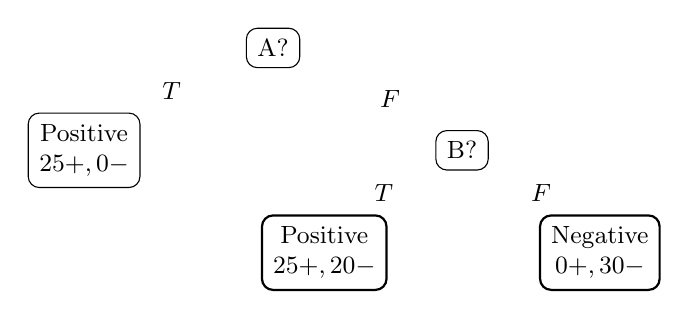
\begin{tikzpicture}[
  level distance=13mm,
  level 1/.style={sibling distance=48mm},
  level 2/.style={sibling distance=35mm},
  every node/.style={draw,rounded corners,align=center,font=\small,inner sep=4pt},
  edge from parent/.style={-{Stealth[length=1.8mm]},thick}
]
\node {A?}
  child {node {Positive\\\(25+,0-\)}
    edge from parent node[left,draw=none,fill=white] {\(T\)}}
  child {node {B?}
    child {node {Positive\\\(25+,20-\)}
      edge from parent node[left,draw=none,fill=white] {\(T\)}}
    child {node {Negative\\\(0+,30-\)}
      edge from parent node[right,draw=none,fill=white] {\(F\)}}
    edge from parent node[right,draw=none,fill=white] {\(F\)}};
\end{tikzpicture}
\caption{Decision tree after selecting \(A\) at the root and \(B\) for the \(A=F\) child.}
\label{fig:decision-tree}
\end{figure}

\section*{Question 3. DBSCAN Clustering}
Use Euclidean distance, \(\varepsilon=2\), and \(\mathrm{MinPts}=2\). \textbf{MinPts includes the point itself.} Thus a point is core if its closed \(\varepsilon\)-neighbourhood contains at least two points, including itself.

\begin{center}
\small
\begin{tabular}{c|l|c|l}
\toprule
Point & \(N_\varepsilon(P)\) & Count & Type\\
\midrule
\(A_1\)&\(\{A_1\}\)&1&Noise\\
\(A_2\)&\(\{A_2\}\)&1&Noise\\
\(A_3\)&\(\{A_3,A_5,A_6\}\)&3&Core\\
\(A_4\)&\(\{A_4,A_8\}\)&2&Core\\
\(A_5\)&\(\{A_3,A_5,A_6\}\)&3&Core\\
\(A_6\)&\(\{A_3,A_5,A_6\}\)&3&Core\\
\(A_7\)&\(\{A_7\}\)&1&Noise\\
\(A_8\)&\(\{A_4,A_8\}\)&2&Core\\
\bottomrule
\end{tabular}
\end{center}
The resulting clusters are \(C_1=\{A_3,A_5,A_6\}\) and \(C_2=\{A_4,A_8\}\). Points \(A_1,A_2,A_7\) are noise. There are no border points: each non-noise point is core.

\begin{figure}[H]
\centering
\begin{minipage}{0.48\linewidth}
\centering
\textbf{\(\varepsilon=2\)}
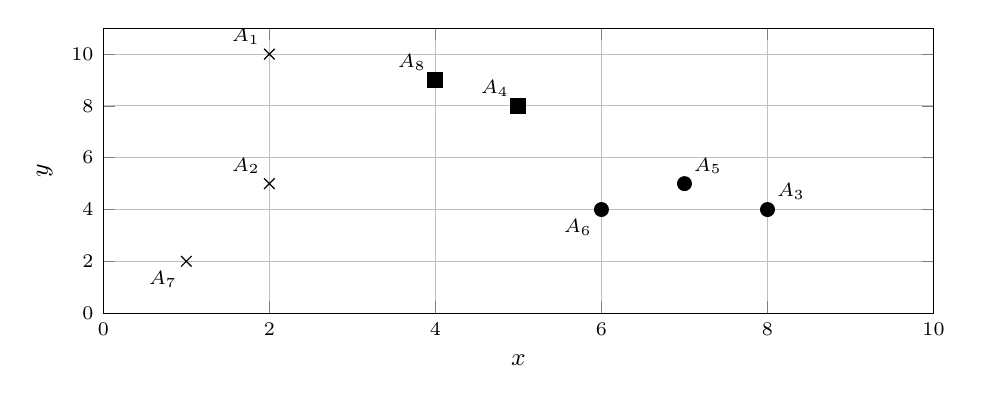
\begin{tikzpicture}
\begin{axis}[
  width=\linewidth,height=5.2cm,
  xmin=0,xmax=10,ymin=0,ymax=11,
  xtick={0,2,4,6,8,10},ytick={0,2,4,6,8,10},
  xlabel=\(x\),ylabel=\(y\),grid=major,
  tick label style={font=\scriptsize},label style={font=\small}
]
\addplot[only marks,mark=*,mark size=2.5pt] coordinates {(8,4)(7,5)(6,4)};
\addplot[only marks,mark=square*,mark size=2.7pt] coordinates {(5,8)(4,9)};
\addplot[only marks,mark=x,mark size=2.7pt] coordinates {(2,10)(2,5)(1,2)};
\node[font=\scriptsize,above left] at (axis cs:2,10) {\(A_1\)};
\node[font=\scriptsize,above left] at (axis cs:2,5) {\(A_2\)};
\node[font=\scriptsize,above right] at (axis cs:8,4) {\(A_3\)};
\node[font=\scriptsize,above left] at (axis cs:5,8) {\(A_4\)};
\node[font=\scriptsize,above right] at (axis cs:7,5) {\(A_5\)};
\node[font=\scriptsize,below left] at (axis cs:6,4) {\(A_6\)};
\node[font=\scriptsize,below left] at (axis cs:1,2) {\(A_7\)};
\node[font=\scriptsize,above left] at (axis cs:4,9) {\(A_8\)};
\end{axis}
\end{tikzpicture}
\end{minipage}\hfill
\begin{minipage}{0.48\linewidth}
\centering
\textbf{\(\varepsilon=10\)}
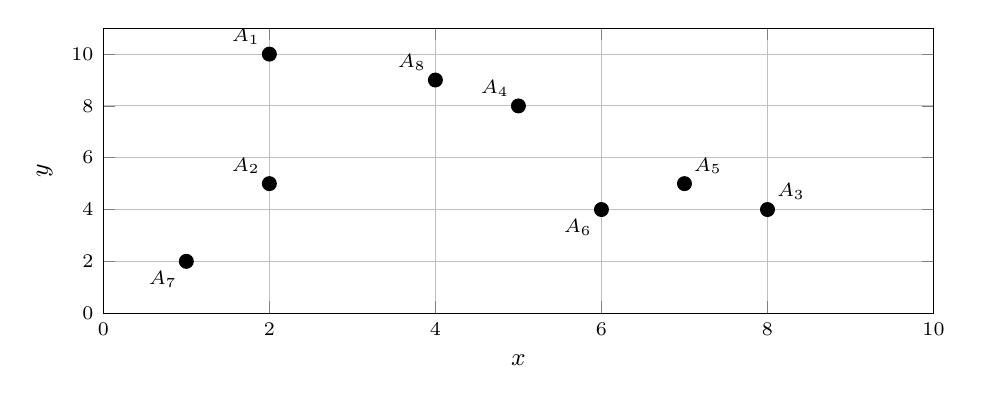
\begin{tikzpicture}
\begin{axis}[
  width=\linewidth,height=5.2cm,
  xmin=0,xmax=10,ymin=0,ymax=11,
  xtick={0,2,4,6,8,10},ytick={0,2,4,6,8,10},
  xlabel=\(x\),ylabel=\(y\),grid=major,
  tick label style={font=\scriptsize},label style={font=\small}
]
\addplot[only marks,mark=*,mark size=2.5pt] coordinates
  {(2,10)(2,5)(8,4)(5,8)(7,5)(6,4)(1,2)(4,9)};
\node[font=\scriptsize,above left] at (axis cs:2,10) {\(A_1\)};
\node[font=\scriptsize,above left] at (axis cs:2,5) {\(A_2\)};
\node[font=\scriptsize,above right] at (axis cs:8,4) {\(A_3\)};
\node[font=\scriptsize,above left] at (axis cs:5,8) {\(A_4\)};
\node[font=\scriptsize,above right] at (axis cs:7,5) {\(A_5\)};
\node[font=\scriptsize,below left] at (axis cs:6,4) {\(A_6\)};
\node[font=\scriptsize,below left] at (axis cs:1,2) {\(A_7\)};
\node[font=\scriptsize,above left] at (axis cs:4,9) {\(A_8\)};
\end{axis}
\end{tikzpicture}
\end{minipage}
\caption{DBSCAN point classifications at \(\varepsilon=2\) and \(\varepsilon=10\).}
\label{fig:dbscan-plots}
\end{figure}

For \(\varepsilon=10\), the greatest pairwise distance is
\(\operatorname{dist}(A_1,A_3)=\sqrt{72}<10\). Every point is therefore in every point's \(\varepsilon\)-neighbourhood; all eight are core and form one cluster, with no border points or noise.
\[
N_{10}(A_i)=\{A_1,A_2,A_3,A_4,A_5,A_6,A_7,A_8\},
\qquad i=1,\ldots,8.
\]

\section*{Question 4. Association Rule Mining}
\subsection*{(a) Confidence and thresholds}
\[
\conf(A\to B)=\frac{\supp(A,B)}{\supp(A)}
=\frac{0.20}{0.25}=0.80=80\%.
\]
The rule support is \(20\%\), above the \(10\%\) minimum, and confidence is \(80\%\), above the \(60\%\) minimum. It passes both thresholds.

\subsection*{(b) Lift}
\[
\Lift(A,B)=\frac{0.20}{0.25(0.90)}
=\frac{0.20}{0.225}\approx0.8889.
\]
Since lift is below 1, \(A\) and \(B\) have a negative association: \(B\) occurs less often with \(A\) than would be expected under independence. Lift equal to 1 indicates independence.

\subsection*{(c) Proof}
Let \(p=\supp(A)\), \(q=\supp(B)\), and \(r=\conf(A\to B)=P(B\mid A)\). Given \(r<q\), and assuming \(0<p<1\), the law of total probability gives
\[
q=pr+(1-p)\conf(\neg A\to B).
\]
Rearrange:
\[
\conf(\neg A\to B)=\frac{q-pr}{1-p}
=q+\frac{p(q-r)}{1-p}.
\]
Here \(p>0\), \(1-p>0\), and \(q-r>0\), so
\[
\conf(\neg A\to B)>q=\supp(B)>r=\conf(A\to B).
\]
This proves both required inequalities. The condition \(p<1\) is necessary for \(\neg A\) to have a defined confidence.

\section*{Question 5. Apriori and FP-Growth}
The minimum support count is \(0.60(5)=3\) transactions.

\subsection*{(a) Frequent itemsets}
Singleton counts are:
\[
\supp(M)=3,\ \supp(O)=3,\ \supp(N)=2,\ \supp(K)=5,\ \supp(E)=4,\ 
\supp(Y)=3,\ \supp(D)=\supp(A)=\supp(U)=\supp(I)=1,\ \supp(C)=2.
\]
Thus \(L_1=\{M,O,K,E,Y\}\).

\begin{center}
\small
\begin{tabular}{c|r@{\qquad}c|r}
\toprule
Candidate pair & Count & Candidate pair & Count\\
\midrule
MO&1& MK&3\\
ME&2& MY&2\\
OK&3& OE&3\\
OY&2& KE&4\\
KY&3& EY&2\\
\bottomrule
\end{tabular}
\end{center}
The frequent pairs are
\[
L_2=\{MK,OK,OE,KE,KY\},
\]
with their counts as shown. After Apriori pruning, the only possible 3-item candidate is \(OKE\), because all its 2-item subsets \(OK,OE,KE\) are frequent. Its support is 3, so \(L_3=\{OKE\}\). No 4-item candidate survives pruning.

\textbf{FP-Growth.} Frequent-item order (descending support, ties alphabetically) is
\(K,E,M,O,Y\). After removing infrequent items and sorting each transaction in this order:
\[
\begin{array}{ll}
T100:K,E,M,O,Y;&T200:K,E,O,Y;\\
T300:K,E,M;&T400:K,M,Y;\\
T500:K,E,O.&
\end{array}
\]
The resulting FP-tree node counts are:

\begin{figure}[H]
\centering
\resizebox{0.9\linewidth}{!}{%
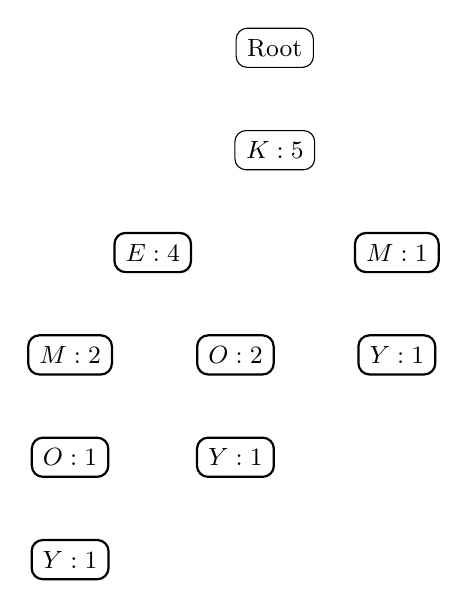
\begin{tikzpicture}[
  every node/.style={draw,rounded corners,inner sep=4pt,font=\small},
  edge from parent/.style={-{Stealth[length=1.7mm]},thick},
  level distance=13mm,
  level 1/.style={sibling distance=50mm},
  level 2/.style={sibling distance=31mm},
  level 3/.style={sibling distance=21mm},
  level 4/.style={sibling distance=18mm}
]
\node {Root}
 child {node {\(K:5\)}
   child {node {\(E:4\)}
     child {node {\(M:2\)}
       child {node {\(O:1\)}
         child {node {\(Y:1\)}}}
     }
     child {node {\(O:2\)}
       child {node {\(Y:1\)}}}
   }
   child {node {\(M:1\)}
     child {node {\(Y:1\)}}
   }
 };
\end{tikzpicture}}
\caption{FP-tree after filtering to frequent items and ordering each transaction.}
\label{fig:fptree}
\end{figure}

FP-Growth returns the same frequent patterns:
\[
L_1=\{M:3,O:3,K:5,E:4,Y:3\},\quad
L_2=\{MK:3,OK:3,OE:3,KE:4,KY:3\},\quad L_3=\{OKE:3\}.
\]
\begin{center}
\small
\begin{tabularx}{\linewidth}{>{\bfseries}p{0.2\linewidth}XX}
\toprule
Algorithm & Main work & Result / efficiency\\
\midrule
Apriori & Generates candidates level by level and scans transactions to count support. & Explicit candidates \(C_1,C_2,C_3\); easy to understand, but repeated scans and candidate generation can be costly.\\
FP-Growth & Builds a compressed FP-tree and mines conditional pattern bases without candidate generation. & Same frequent itemsets; typically fewer repeated scans and no large explicit candidate sets.\\
\bottomrule
\end{tabularx}
\end{center}

\subsection*{(b) Strong rules matching \(\{item_1,item_2\}\to\{item_3\}\)}
The only frequent triple is \(OKE\), with support \(3/5=60\%\). Its three possible rules are:
\[
\begin{array}{c|c|c|c}
\text{Rule}&\text{Support}&\text{Confidence}&\text{Meets both thresholds?}\\ \hline
\{O,K\}\to\{E\}&3/5=60\%&3/3=100\%&\text{Yes}\\
\{O,E\}\to\{K\}&3/5=60\%&3/3=100\%&\text{Yes}\\
\{K,E\}\to\{O\}&3/5=60\%&3/4=75\%&\text{No: confidence}<80\%
\end{array}
\]
Therefore, the complete strong-rule set is
\(\boxed{\{O,K\}\to\{E\},\ \{O,E\}\to\{K\}}\).

\section*{Question 6. Contingency Tables and Interestingness Measures}
The ten transactions in Table 6.4 of the supplied PDF are transcribed as
\[
\begin{array}{c|l@{\qquad}c|l}
1&\{a,b,d,e\}&2&\{b,c,d\}\\
3&\{a,b,d,e\}&4&\{a,c,d,e\}\\
5&\{b,c,d,e\}&6&\{b,d,e\}\\
7&\{c,d\}&8&\{a,b,c\}\\
9&\{a,d,e\}&10&\{b,d\}
\end{array}
\]
For each rule, table rows indicate antecedent present/absent and columns indicate consequent present/absent.

\small
\begin{center}
\textbf{Rule 1: \(\{b\}\to\{e\}\)}
\begin{tabular}{c|rr}
&\(e\)&\(\neg e\)\\\hline
\(b\)&\(n_{11}=4\)&\(n_{10}=3\)\\
\(\neg b\)&\(n_{01}=2\)&\(n_{00}=1\)
\end{tabular}

\vspace{4pt}
\textbf{Rule 2: \(\{a\}\to\{d\}\)}
\begin{tabular}{c|rr}
&\(d\)&\(\neg d\)\\\hline
\(a\)&\(n_{11}=4\)&\(n_{10}=1\)\\
\(\neg a\)&\(n_{01}=5\)&\(n_{00}=0\)
\end{tabular}

\vspace{4pt}
\textbf{Rule 3: \(\{b\}\to\{d\}\)}
\begin{tabular}{c|rr}
&\(d\)&\(\neg d\)\\\hline
\(b\)&\(n_{11}=6\)&\(n_{10}=1\)\\
\(\neg b\)&\(n_{01}=3\)&\(n_{00}=0\)
\end{tabular}

\vspace{4pt}
\textbf{Rule 4: \(\{c\}\to\{e\}\)}
\begin{tabular}{c|rr}
&\(e\)&\(\neg e\)\\\hline
\(c\)&\(n_{11}=2\)&\(n_{10}=3\)\\
\(\neg c\)&\(n_{01}=4\)&\(n_{00}=1\)
\end{tabular}

\vspace{4pt}
\textbf{Rule 5: \(\{c\}\to\{a\}\)}
\begin{tabular}{c|rr}
&\(a\)&\(\neg a\)\\\hline
\(c\)&\(n_{11}=2\)&\(n_{10}=3\)\\
\(\neg c\)&\(n_{01}=3\)&\(n_{00}=2\)
\end{tabular}
\end{center}
\normalsize

\textbf{(b) Missing measure list in source.} Page 3 of the supplied PDF says to rank the rules according to ``the following measures,'' but the measures themselves are absent from the page image/text before Question 7 begins. Since the assignment does not identify which measures to use, no ranking is fabricated. The five contingency tables above provide the counts needed once the intended measures are supplied.

\section*{Question 7. Classification of Breast Tumours}
The dataset has five benign and five malignant samples. For Gaussian Naive Bayes, use the class-wise maximum-likelihood (population) variances and conditional independence of \(X_1,X_2\) given the diagnosis.

\subsection*{(a) Gaussian Naive Bayes}
The priors are \(P(B)=P(M)=5/10=0.5\). For a Gaussian feature,
\[
f(x\mid\mu,\sigma^2)=\frac{1}{\sqrt{2\pi\sigma^2}}
\exp\left(-\frac{(x-\mu)^2}{2\sigma^2}\right).
\]

\begin{center}
\small
\begin{tabular}{c|cc|cc}
\toprule
Class & \(\mu_{X_1}\)&\(\sigma^2_{X_1}\)&\(\mu_{X_2}\)&\(\sigma^2_{X_2}\)\\
\midrule
B &13.8&0.86&0.060&0.000200\\
M &16.8&0.86&0.172&0.000976\\
\bottomrule
\end{tabular}
\end{center}
For the test point \(X=(15.8,0.12)\), the feature likelihoods and unnormalized posteriors are:
\[
\begin{array}{c|rrr}
&f(15.8\mid X_1)&f(0.12\mid X_2)&P(\text{class})\prod_j f(x_j\mid\text{class})\\ \hline
B&0.042041&0.003481&0.00007318\\
M&0.240527&3.195807&0.384339
\end{array}
\]
Normalizing the last column gives
\[
P(B\mid X)\approx0.000190,\qquad
P(M\mid X)\approx0.999810.
\]
Hence the predicted class is \(\boxed{M\text{ (Malignant)}}\).

\subsection*{(b) Bayesian Network}
The DAG is \(X_1\to X_2,\ X_1\to D,\ X_2\to D\), where \(D\) is diagnosis.
\(X_1\) has no parents and children \(X_2,D\); \(X_2\) has parent \(X_1\) and child \(D\); \(D\) has parents \(X_1,X_2\) and no children.

\begin{figure}[H]
\centering
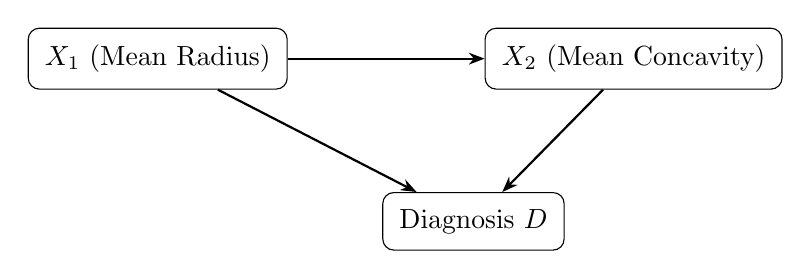
\begin{tikzpicture}[node distance=25mm,every node/.style={draw,rounded corners,inner sep=6pt}]
\node (x1) {\(X_1\) (Mean Radius)};
\node (x2) [right=of x1] {\(X_2\) (Mean Concavity)};
\node (d) [below right=13mm and 12mm of x1] {Diagnosis \(D\)};
\draw[-{Stealth[length=2mm]},thick] (x1)--(x2);
\draw[-{Stealth[length=2mm]},thick] (x1)--(d);
\draw[-{Stealth[length=2mm]},thick] (x2)--(d);
\end{tikzpicture}
\caption{Specified Bayesian network structure.}
\label{fig:bayesian-network}
\end{figure}

Apply the specified thresholds: \(X_1=L\) for \(X_1<15\), otherwise \(H\);
\(X_2=L\) for \(X_2<0.10\), otherwise \(H\). Thus \(X_1\) has 4 L and 6 H observations; \(X_2\) has 5 L and 5 H.
With Laplace smoothing \(\alpha=1\), the root prior and \(X_2\mid X_1\) CPTs are:
\[
\begin{array}{c|cc}
X_1&L&H\\ \hline
\text{Count}&4&6\\
P(X_1\mid\text{root})&5/12&7/12
\end{array}
\qquad
\begin{array}{c|r r|cc}
X_1&n(X_2=L)&n(X_2=H)&P(L\mid X_1)&P(H\mid X_1)\\ \hline
L&4&0&5/6&1/6\\
H&1&5&1/4&3/4
\end{array}
\]
For \(D\mid X_1,X_2\), add one to each of the two diagnosis-class counts in every parent configuration:
\[
\begin{array}{cc|rr|cc}
X_1&X_2&n(B)&n(M)&P(B\mid X_1,X_2)&P(M\mid X_1,X_2)\\ \hline
L&L&4&0&5/6&1/6\\
L&H&0&0&1/2&1/2\\
H&L&1&0&2/3&1/3\\
H&H&0&5&1/7&6/7
\end{array}
\]
The query sample is \(X_1=H,X_2=H\), so
\[
\boxed{P(D=M\mid X_1=H,X_2=H)=6/7\approx0.8571.}
\]
The edge \(X_1\to X_2\) represents their dependence: in this sample, \(P(X_2=H\mid X_1=H)=3/4\), whereas \(P(X_2=H\mid X_1=L)=1/6\).

\subsection*{(c) Linear SVM}
Use original, unscaled features and a hard-margin linear SVM; the labels are linearly separable. The nearest opposite-class observations are \(S5=(15,0.07)\) with label \(-1\) and \(S6=(15.5,0.13)\) with label \(+1\). Their difference is
\[
d=S6-S5=(0.5,0.06).
\]
Under the canonical constraints \(y_i(w^\top x_i+b)\geq1\),
\[
w=\frac{2d}{\|d\|^2}
=\left(\frac{1}{0.2536},\frac{0.12}{0.2536}\right)
\approx(3.943218,0.473186).
\]
The separating line passes through the midpoint \((15.25,0.10)\), hence
\[
b=-w^\top(15.25,0.10)\approx-60.181388,
\]
\[
\boxed{f(X)=3.943218X_1+0.473186X_2-60.181388=0.}
\]
Equivalently, a positive scalar multiple is \(0.5X_1+0.06X_2-7.631=0\).
The support vectors are \(S5,S6\), where \(f(S5)=-1\) and \(f(S6)=+1\).
The vector norm and margin values are
\[
\|d\|_2^2 = (0.5)^2 + (0.06)^2 = 0.2536
\]
\[
\|d\|_2 = \sqrt{0.2536} \approx 0.503588
\]
The margin width between support hyperplanes is
\[
\frac{2}{\|w\|_2} = \|d\|_2 \approx 0.503588
\]
The distance from the separating hyperplane to either margin is
\(1/\|w\|\approx0.251794\).
For \(X=(15.8,0.12)\),
\[
f(X)\approx2.178233>0,
\]
so the SVM predicts \(\boxed{M\text{ (Malignant)}}\).

\begin{figure}[H]
\centering
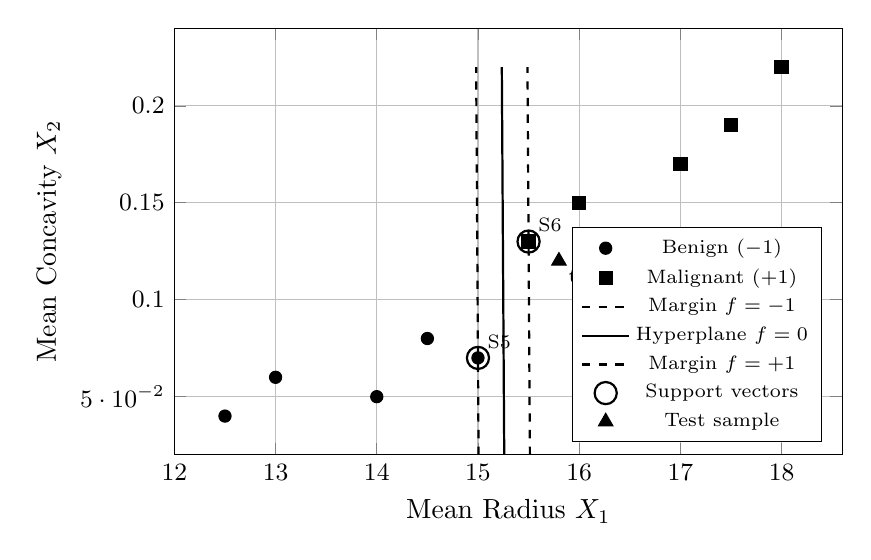
\begin{tikzpicture}
\begin{axis}[
  width=0.83\linewidth,height=7.0cm,
  xmin=12,xmax=18.6,ymin=0.02,ymax=0.24,
  xlabel={Mean Radius \(X_1\)},ylabel={Mean Concavity \(X_2\)},
  grid=major,legend pos=south east,
  legend style={font=\scriptsize,draw=black,fill=white},
  tick label style={font=\small}
]
\addplot[only marks,mark=*,mark size=2.2pt] coordinates
  {(12.5,0.04)(13,0.06)(14,0.05)(14.5,0.08)(15,0.07)};
\addlegendentry{Benign (\(-1\))}
\addplot[only marks,mark=square*,mark size=2.4pt] coordinates
  {(15.5,0.13)(16,0.15)(17,0.17)(17.5,0.19)(18,0.22)};
\addlegendentry{Malignant (\(+1\))}
\addplot[black,dashed,thick] coordinates {(15.0060,0.02)(14.9820,0.22)};
\addlegendentry{Margin \(f=-1\)}
\addplot[black,thick] coordinates {(15.2596,0.02)(15.2356,0.22)};
\addlegendentry{Hyperplane \(f=0\)}
\addplot[black,dashed,thick] coordinates {(15.5132,0.02)(15.4892,0.22)};
\addlegendentry{Margin \(f=+1\)}
\addplot[only marks,mark=o,mark size=4pt,thick] coordinates {(15,0.07)(15.5,0.13)};
\addlegendentry{Support vectors}
\addplot[only marks,mark=triangle*,mark size=3pt] coordinates {(15.8,0.12)};
\addlegendentry{Test sample}
\node[font=\scriptsize,anchor=south west] at (axis cs:15,0.07) {S5};
\node[font=\scriptsize,anchor=south west] at (axis cs:15.5,0.13) {S6};
\node[font=\scriptsize,anchor=north west] at (axis cs:15.8,0.12) {test};
\end{axis}
\end{tikzpicture}
\caption{Original-scale observations, hard-margin SVM boundary, margins, and support vectors.}
\label{fig:svm}
\end{figure}

\end{document}
